\chapter{Introduction}\label{ref:chp1}

% In this chapter, we introduce the fundamentals of genetics and DNA sequencing. Furthermore, we introduce the important research problem in the field of genetics, the diploid genome assembly (haplotyping). 
% We will see how we can mathematically formualate the diploid assembly problem as a computer scientist.
% Then we provide a high level description of the main methods used in this problem.
% Thereafter, we describe the limits and challenges faced currently in this field. We finish this chapter by an outline of the thesis.


Genetics and Genomics study the phenomenon of \textit{life} at its most basic level and are like wise fascinating and important.
% In this section we describe the basics about genetics and haplotyping. We provide motivation about why understanding genetics for different organisms is so important.
% https://www.gen.cam.ac.uk/undergraduate/whygenetics
% http://www.helsinki.fi/biosciences/genetics/
An important field in genetics is haplotyping.
Haplotyping is the process of determining the sequences of both copies of homologous chromosomes, which are inherited from each parent in diploid organisms.
Haplotyping has applications in different fields such as evolutionary studies, clinical diagnosis, precision medicine, and biotechnology. 
Third generation sequencing technologies allow for reading fragments (in the order of magnitude of tens of kilo-bases) of the genome sequence, and thus the reconstruction of haplotypes is
possible, in principle. Unfortunately, sequencing is prone to errors and the use of advanced algorithms and models is essential to correct for errors, in order to reconstruct accurate haplotypes.
However, the process of correcting these errors poses various computational challenges.
In this thesis, we present novel algorithms to addressing various computational challenges in this field.

\section{Genetics, DNA sequencing and Haplotyping}\label{sec:dna_seq}
Genetics is the study of genes, genetic variation, and heredity in living organisms. 
Genetics controls what an organism looks like and how it functions.
% The DNA is the carrier of hereditary information and thus understanding DNA in detail has been the central aim for many researchers.
% Classically the genetic variants (mutations) present in the living organisms have been used to study and investigate the cause of biological diseases and, additionally helps to make deductions about the way cells and organisms worked. 
% Genetics is the study of genes, genetic variation, and heredity in living organisms.
Specifically, there are two sides to the science of genetics.
On the one hand, the availability of different types of molecular information, such as sequence information and gene expression levels, paired with gene editing techniques with which we can perturb the genome in a controlled fashion and observe its biological effects, 
provides powerful explanation tools to the functions of genes.
On the other hand, genetics provides a fundamental understanding of how organisms, populations, and species evolve. 
In the last few years, one of the most exciting new developments is the way in which these two sides have begun to converge \citep{casillas2017molecular}.
This convergence is achieved through the development of technologies that provide datasets from the genomic level to epigenomic, transcriptomic or proteomics level.
% The integrative analyses of these datasets promise to provide a systematic view of the causes and consequences of evolution, development and functions of organisms.

% these vary during the lifetime of the individual, therefore, have the potential to provide insights  effort of using molecular techniques to understand the processes of development, evolution, and speciation.
% % Modern computational biology tools (analysis of genomic sequences and bioinformatics) use these integrative principles 
% % to answer various difficult biological questions ranging from the mechanisms of evolution to the development of complex diseases.
% Thus, genetics has a central role in modern biology and its influence is ever increasing.

% s\todo{citations are missing in this para or even figures.}
% from italy person thesis.
% \textit{What actually is genetic information?} 
The discovery of the double helix structure of deoxyribonucleic acid (DNA) by Watson and Crick in 1953 laid the main foundation for modern genetics.
In most living organisms, genetic information is encoded in the form of DNA molecules.
A DNA molecule is a chain in which many bases are ordered in a linear sequence, the bases --- A, T, G, and C --- are the letters of the genetic alphabet.
The whole information within the DNA molecules of an organism is called its genome. The genome is divided into chromosomes.
Genomes have single (haploid), double (diploid) or higher ploidy with more than two homologous chromosomes (polyploids). 
In this thesis, we focus on \textit{diploid} organisms. For example, humans are diploids, consisting of two copies of each chromosome called homologous chromosomes or \textit{haplotypes} --- one inherited from the mother and the other from the father.
There are differences between these two copies of each chromosome known as genetic variation. 
% \todo{this para explained in more detail in biological background.}

In the early 2000s, a historic breakthrough happened with the sequencing of the human genome \citep{venter2001sequence, collins2003human}.
Moreover, sequencing datasets of the human genome are made available as open-access to help in their interpretation and understanding \citep{church2005personal}.
Specifically, \textit{sequencing} is an operation that determines the base sequence of a DNA molecule.
For sequencing genomes, there exist several kinds of sequencing technologies which share the following common properties.
First, they yield genomes in fragments called ``reads''. Second, the position of reads along the genome sequence is unknown and also, mostly, the strand from which the read was sampled is unknown.
Third, the reads contain errors.

% Huge amounts of sequencing data are routinely produced by next generation sequencing technologies (NGS).  The major challenge with these sequencing datasets is that genomic information is partial and erroneous. 
Sequencing technologies differ in terms of error rates and lengths of the produced reads. We define the error rate of a read as the ratio of the number of incorrectly sequenced bases to the length of the read.
Broadly, the sequencing technologies can be categorized into three classes:
\begin{itemize}
\item First generation sequencing: The first sequencing technologies were developed in 1977 by \cite{sanger1977dna}, who is awarded a Nobel Prize in chemistry, and \cite{maxam1977new}.
Sanger sequencing produces reads in the order of 800-1000 base pairs with an error rate $\le 1$\%.
 \item Second generation sequencing: It includes Illumina/Solexa sequencing \citep{bentley2008accurate}, which has been the most widespread technology. 
 This technology produces short reads (hundreds of bases) with an error rate $\le 1$\%. 
  \item Third generation sequencing: It includes Single Molecule Real Time sequencing (PacBio) \citep{eid2009real} 
  and Oxford Nanopore sequencing (ONT) \citep{laszlo2014decoding}. These technologies produce very long sequences that are up to hundreds of kilo-bases in length. 
  The downside is that PacBio and ONT exhibit very high error rates of up to 15\% and 38\% respectively. 
  %   \item Synthetic long read sequencing: This technology includes 10x Genomics technology \citep{eisenstein2015startups}, which adds a unique barcode to every short read (produced from Illumina platform) generated from an individual molecule. 
%   The barcode information allows to link short reads together at a long-range and the linked-read length is ~50 kb.
%  \item Single-cell sequencing: This technology includes Strand specific sequencing (Strand-Seq), which produces Illumina reads, along with information on the directionality of DNA. Each single strand of a DNA molecule is labeled regarding its 5'–3' orientation \citep{falconer2012dna}.
\end{itemize}

Furthermore, there exist some sequencing protocols that provide long-range information.
One of the sequencing protocols is the Strand specific protocol (Strand-Seq), which includes preparation of single-cell libraries. 
Also, each single strand of a DNA molecule is labeled regarding its 5'–3' orientation \citep{falconer2012dna}.
Illumina sequencing is performed from parental template strands in these single-cell libraries.
The sequencing results in Illumina reads, along with information on the directionality of DNA. 
The other sequencing protocol is the 10x Genomics protocol \citep{eisenstein2015startups}, which adds a unique barcode to every short read (produced from Illumina platform) generated from an individual molecule.

% Furthermore, each sequencing technology has some bias due to the protocols employed.
% The high G/C content regions are sequenced less frequently by the short read technologies than the rest of the genome and the downstream end of reads exhibit a high error rate \citep{aird2011analyzing, dohm2008substantial}.

% Huge amounts of sequencing data are routinely produced by these sequencing technologies.
Sequencing data is routinely used to reconstruct the underlying haplotypes for diploid genomes. Reconstructing haplotypes is required in order to correctly understand allele-specific expression and compound heterozygosity. 
Compound heterozygosity is the phenomenon when the two homologous copies of a genomic region each contain unique sequence variants, 
but at different positions in that region. These variants are responsible for different functioning of the two homologous copies of a gene, resulting in different phenotypes.
Thus, in settings in which compound heterozygosity play a role, the knowledge about the specific haplotype is essential.
Haplotypes also help in investigating the genetic determinants of common diseases, and in performing population-genetic analyses of admixture, migration and selection \citep{tewhey2011importance, Glusman2014}. 
Furthermore, haplotype sequences are used in relating genotypes to phenotypes, and for understanding how the arrangement of cis- and trans-acting variants across the two homologous copies of a genomic region affects phenotypic expression.

Technological progress in sequencing and computational approaches has enabled the reconstruction of underlying haplotypes for diploid genomes.
However, there are intrinsic benefits and challenges when utilizing sequencing reads from different sequencing technologies. 
Specifically, upcoming PacBio and ONT sequencing deliver long reads, but have high sequencing error rates.
In contrast, Illumina sequencing delivers reads with low error rates, but have short lengths. Currently, no sequencing technology delivers data that is complete and non-erroneous.
Thus, the reconstruction of accurate and complete haplotypes (without gaps) from sequencing datasets remains a challenging problem.
% Specifically, upcoming long-read technologies deliver reads that span multiple variants and therefore, provide power to connect multiple variants into blocks, 
% leading to reconstruct the whole genome.
% The challenge of long-read technologies is high sequencing error rates. 
% % To overcome this challenge, the long noisy sequencing datasets are often supplemented with short accurate datasets.
% One potential way to generating complete and accurate genomes could be to combine multiple sequencing technologies, one that produces long reads with high error rates and other that produces 
% short reads with low error rates.

% \textit{What are the other challenges across all technologies in producing a diploid genome?}
From available sequencing datasets, the first challenge for reconstructing haplotypes arises from a lack of information of the genomic location of reads.
The next challenge is the lack of the \textit{haplotypic identity} of reads, i.e.\, the haplotype that the read comes from.
Knowing the haplotype of reads is essential for reconstructing both copies of each chromosome, which in turn helps better understand the true biological characteristics of diploid organisms.
% Thus, from the biological point of view, the single individual haplotyping (SIH) problem consists in the reassignment of each read to the original haplotype.
% Once we know this identity, it becomes easier to assemble the reads from each haplotype separately to further reconstruct the two genome sequences of diploid organisms.
% The process of reconstructing the diploid assemblies from sequencing reads is known as \textit{diploid genome assembly} or \textit{haplotyping}.


\begin{figure}[t!]\centering
\includegraphics[width=\columnwidth]{{ex1-intro1}.pdf}
\caption{Seven variants covered by reads (horizontal bars) in a single individual.
The alleles that a read supports are printed in white. The middle panel shows the phased reads in colors and haplotypes at the bottom over the seven variants.}
\label{fig:ex1_intro}
\end{figure}

\vspace{10cm}
The clever approaches are developed to solve these challenges. Broadly, the approaches to obtain haplotypes are classified into two categories: \textit{reference-based} haplotyping and \textit{haplotype-aware de novo} assembly.

% This absence of context and the small size and error rates of the sequences obtained, relatively to the genome size, makes it difficult to use reads as such.
% Ideally, we would need the access to the underlying genomes in their entirety.
% Since the beginning of sequencing of DNA molecules, genomes are produced by structuring and ordering reads information. 
% Then these reconstructed genomes can be used
% as references. 
% Reference genomes provide reliable information on the genomic location of reads. 
% Over the years, a lot of effort has been devoted to generating good quality reference genomes.
%  Reference genomes reveal the organization of the genome,
% including the relative position of genes or chromosomes structure \citep{encode2004encode}. 
% Reference genomes have been used by biologists for other tasks, for instance, finding the functions to annotate the genome \citep{harrow2012gencode}.

% Reference genome can be used to identifying the location of origin of each read.
% To this end, we align them to the reference genome. 
% The aligned reads are then partitioned into two sets to generate haplotypes. This process is called \textit{reference-based} haplotyping (phasing) or single individual haplotyping or read-based phasing.

% In reference-based haplotyping, read mapping step has a reference bias because the reference genome does not capture the genomic diversity of a population.
% The reads that are unique to the target genome, are not aligned or wrongly aligned to the reference genome.
% The usage of reference genomes for read alignment hence generate a bias. This reference bias causes problems for further downstream analyses. 
% To overcome these problems, the approach that uses reference genomes is generalized in order to perform \textit{haplotype-aware de novo} assembly.

% In \textit{haplotype-aware de novo} assembly, the reference genome is not used, but the haplotypes are instead constructed directly from the reads.
% In a reference-based approach, the reads are aligned to the reference genome and then the aligned reads are partitioned into two sets to generate the haplotypes.
% This process is 
% To determine the assignment of each read to one of the homologous copies of chromosome (haplotype) is an important question. 
% Thus, from the biological point of view, the haplotyping (SIH) problem consists in the reassignment of each read to the original haplotype.
% Once we know this identity, it becomes easier to assemble the reads from each haplotype separately to further reconstruct the two genome sequences of diploid organisms.
% The process of reconstructing the diploid assemblies from sequencing reads is known as \textit{diploid genome assembly} or \textit{haplotyping}.

% These approaches for haplotyping are discussed below in detail (Sections \ref{sec:ref} and \ref{sec:dip}). 
% First, we present formulation and methods to solving reference-based haplotyping (single individual haplotyping) and then explain the generalized approach for performing \textit{haplotype-aware} de novo assembly.
\section{Reference-based Haplotyping}\label{sec:ref}
\textit{Reference-based} phasing methods are applied when a reference genome is available for the species of the target genome.
We expect the target genome to be very close to the reference, more specifically, given the reads of the target genome, we expect the reference to be from the same species as the reads.
% We are interested to phase the differences of target genome to its reference.

Reference genomes provide reliable information on the genomic location of reads. 
Over the years, a lot of effort has been devoted to generating good quality reference genomes \citep{10002010map, international2005haplotype}.
 Reference genomes provide the organization of the genome,
including the relative position of genes or chromosomes structure \citep{encode2004encode}. 
Reference genomes have been used by biologists for other tasks, for instance, finding the functions to annotate the genome \citep{harrow2012gencode}.

Standard pipelines for reference-based phasing consist of the following steps: 
First, the reads are aligned to the reference genome. Second, the variants are detected using various variant calling algorithms, to finding the differences of target genome to the reference.
Third, the detected variants are phased based on how aligned reads connect the alleles over them, to generate two haplotypes.

Please note that the different terminologies \textit{reference-based} haplotyping (phasing), single individual haplotyping and read-based phasing are used interchangeably in this thesis.

% The main focus of this study is the third step in the pipeline.
% For illustration, the toy example is given in Figure~\ref{fig:ex1_intro}.


 To illustrate the haplotyping problem for a single genome, we consider a small example in Figure~\ref{fig:ex1_intro}. The example shows seven variants. Also shown are the sequencing reads aligned to the reference genome.
 The alleles that the reads support are shown in white. 
 Erroneous alleles in the reads are shown in red. In practice, we do not know the alleles that contain these sequencing errors. 
 The goal of the \textit{reference-based} haplotyping problem is the re-assignment of phases to the reads, i.e.\, assigning haplotype-specific colors (green or purple) to each read. 
 In the middle panel, the colored bars represent the assignment of each read to either the green or the purple haplotype.
 Finally, the reads from each haplotype are separately assembled together in order to output two haplotypes that are shown at the bottom in purple and green.

% In this study, we identify the limitations of the existing methods in phasing a single genome. To overcome these limitations, we propose a novel efficient algorithm.

% you may refer also this: http://homolog.us/Tutorials/index.php?p=1.4&s=1

\subsection{Haplotyping as a Combinatorial Optimization problem}
% For diploid genomes, large volumes of sequencing data, which contain errors, are generated every day. Extracting useful information from these datasets to understand the biology of diploid genomes is a challenging problem. 

% The objective of extracting useful information from noisy data in order to achieve the best possible value of goal, or objective, 
% requires formulating an \textit{optimization} problem, that is defined as: 

% Reference genome reconstruction is therefore crucial in various domains where raw,
% out of context reads are unusable. The task of reordering the reads to reconstruct the
% sequenced genome for diploid organisms is called diploid genome assembly or haplotyping.
% Over the genome, there are difference between two copes for each chromosome, known as variants \todo{explained in biological background}. 
% Traditionally, there are two ways to solve it, one is based on the ordered reads to the reference genome and the other one is \textit{denovo assembly}.
% As it will be detailed further, diploid genome assembly is especially complex as the bases distribution is far
% from being uniform. Genomes present specific patterns such as large repeated sequences
% (repeats), regions with very specific distributions of nucleotides or extremely repeated
% sequences of nucleotides. Such patterns make genomes different from a uniformly distributed sequence of nucleotides. \todo{[13]} shows that a human genome is largely constituted
% of repeated sequences of significant lengths.


% \fbox{\begin{minipage}{30em}
%  In summary, the core messages of DNA, sequencing and haplotyping:
%  \begin{itemize}
%   \item The molecular information of the genomes can be obtained using different sequencing technologies.
%   \item The sequencing data is big, erroneous and not complete.
%   \item The task of recovering the genome sequences for diploid organisms is called as diploid genome assembly or haplotyping.
%  \end{itemize}
% \end{minipage}}
We will see how we can formulate the haplotyping problem as combinatorial optimization problem, that is, 
given an object $\math{o}$, find a solution such that an optimization criterion $\math{f}$ is either minimized or maximized.

For the haplotyping problem, which consists of determining the \textit{haplotypic identity} of each read, we consider the reads that are aligned to reference genome.
A read aligner maps the reads to the reference genome, ideally to positions with a high similarity score for the read. 
The number of read alignments that cover a position is known as the coverage for that position.
Furthermore, we have structural nucleotide variants (SNVs) detected using different variant calling algorithms.
In the case of bi-allelic variants, that is, those variants for which two different alleles are known, three genotypes are possible.
The reference allele is typically denoted as 0 and the alternative allele as 1. Using this
notation, the two chromosomal copies either both carry the reference allele (genotype
0/0), or alternative allele (genotype 1/1) or one of them contains the reference while
the other one carries the alternative allele (genotype 0/1). If both chromosomal copies
carry the same allele (i.e. genotype 0/0 or 1/1), the genotype is called homozygous, while
genotype 0/1 is referred to as heterozygous.
s
Given the variants and the alignments, the goal here is to phase the variants and generate the haplotypes.
% The variants over the genome can be phased by using reads aligned to the reference genome. This process is known as \textit{read-based phasing} or \textit{single individual haplotyping}.

Mathematically, the aligned reads over the variants are encoded in the form of a SNP matrix.
The SNP matrix for the example given in Figure~\ref{fig:ex1_intro} is illustrated in Figure~\ref{fig:ex1_intro1}.
The SNP matrix $\mathcal{F}$ is an element of $\{0,1,-\}^{R\times M}$, where $R$ is the number of reads and $M$ is the number of variants along a chromosome.
Each matrix entry $\mathcal{F}(j,k)$ is $0$ (indicating that the read matches the reference allele) or $1$, indicating that the read matches the alternative allele if the read covers that position and ``$-$'' otherwise.
Note that the ``$-$'' character can also be used to encode the unsequenced ``internal segment'' of a paired-end read.
The goal of the haplotype assembly problem is to generate two haplotypes $h^0,h^1\in\{0,1\}^M$. 

\begin{figure}[t!]\centering
\includegraphics[width=\columnwidth]{{ex1-intro}.pdf}
\caption{Example shows the SNP matrix for the example shown in Fig.~\ref{fig:ex1_intro}. Seven variants covered by reads (horizontal bars) in a single individual.
 The allele in read is encoded as 1 if it matches the allele in the reference position at that position and 0 otherwise.
 The middle panel shows the phased reads in colors and haplotypes at the bottom over these seven variants.}
\label{fig:ex1_intro1}
\end{figure}

The presence of sequencing and mapping errors makes the haplotype assembly problem a challenging task. 
Computationally, this problem has been generally modeled as an optimization problem to correct the sequencing and mapping errors.
In literature, different combinatorial formulations of the problem have been
proposed \citep{lippert2002algorithmic}. Among them, Minimum Error Correction (MEC) \citep{lippert2002algorithmic} has
been proven particularly successful in the reconstruction of accurate haplotypes for
diploid species \citep{martin2016whatshap, he2010optimal, CDW13_exact, Glusman2014, rhee2016survey}. MEC aims to correct the input data with the minimum
number of corrections to the SNP values, such that the resulting reads can be partitioned into two sets, with each set identifying a haplotype. 
To mathematically formulate the minimum number of corrections (MEC) as an optimization problem, we require a few definitions.

The quality of a solution relies on the measure $d(r_1,r_2)$ based on the Hamming distance between any two rows $r_1,r_2\in\{0,1, -\}^M$ in $\mathcal{F}$.
\begin{definition}[Distance] 
 Formally, the distance between rows $r_1$ and $r_2$ is given by
\[d(r_1,r_2):= \big|\big\{k\,\big|\,r_1(k)\neq -\ \wedge\ r_2(k)\neq -\ \wedge\ r_1(k)\neq r_2(k)\big\}\big|.\]
\label{eq:distance}
\end{definition}

\begin{definition}[Feasibility]
A SNP matrix $\mathcal{F}\in\{0,1,-\}^{R\times M}$ is called \emph{feasible} if there exists a bi-partition of rows (i.\,e., reads) into two sets such that all pairwise distances of two rows within the same set are zero.
\label{def:feasible-mec}
\end{definition}
Feasibility of a matrix $\mathcal{F}$ is equivalent to the existence of two haplotypes $h^0,h^1\in\{0,1\}^M$ such that every read $r$ in the matrix has a distance of zero to $h^0$ or to $h^1$ (or both).
The MEC problem can now simply be stated in terms of flipping bits in $\mathcal{F}$, where entries that are $0$ or $1$ can be flipped and ``$-$'' entries remain unchanged.

\begin{problem}[MEC]
Given a matrix $\mathcal{F}\in\{0,1,-\}^{R\times M}$, flip a minimum number of entries in $\mathcal{F}$ in order to obtain a feasible matrix.
\label{prob:mec}
\end{problem}


\begin{definition}[MEC cost]
The MEC cost for a solution $h^0,h^1\in\{0,1\}^M$ is given by: \\
    \[\cost_{\mathcal{F}}(h^0,h^1) := \sum_{i=1}^{n} \min\{\dist(r_i,h^0), \dist(r_i,h^1)\}\]\,.

where $r_i \in \{0,1, -\}^M$ is the $i$-th row of a SNP matrix $\mathcal{F}$.
\label{eq:cost}
\end{definition}

The MEC problem is NP-hard \citep{Cilibrasi2007}, but more detailed analyses require a more fine grained distinction between different instances types, which are described as follows.
\begin{itemize}
 \item $\MEC$: Instances in which entries in each of the $n$ rows of $\mathcal{F}$ are from $\{0,1,-\}$. There is no restriction on the placement of entries $0, 1$ and $-$. These instances are generated from Illumina, 10x Genomics and Strand-Seq sequencing technologies.
 \item $\GMEC$: A \MEC instance is called \emph{gapless} if the entries in each of the $n$ rows of $\mathcal{F}$ follows a regular expression of the type \texttt{$-^*\{0,1\}^*-^*$}. 
 These instances are generated from PacBio, ONT and single-end Illumina like technologies.
 \item $\BMEC$: Instances in which entries in each of the $n$ rows of $\mathcal{F}$ are from $\{0,1\}$ with no gaps.
\end{itemize}

% We now illustrate these \MEC instances for a single genome from different sequencing technologies through an example.

Figure~\ref{fig:ex_MECs} shows an example of a mathematical representation of reads from different sequencing technologies, that cover seven variants. 
 The top panel shows a general \BMEC instance consisting of binary values with no gaps, the middle panel shows a \GMEC instance with binary values in between and gaps at its two ends and, the bottom is 
a \MEC instance which consists of binary values and gaps with no restriction on placement of gaps.




\begin{figure}[t!]\centering
\includegraphics[width=\columnwidth]{{ex-MECs}.pdf}
\caption{Seven variants covered by reads (horizontal bars) in a single individual are represented as \MEC instances. At the top is a general \MEC instance with arbitrary gaps, the middle is a \GMEC instance with gaps only at its two ends and the bottom is 
a \BMEC instance which consists of only binary values.}
\label{fig:ex_MECs}
\end{figure}

Additionally, we consider a weighted version of the MEC (wMEC), in which a cost is associated to every matrix entry.
This is useful in practice since each nucleotide in a sequencing read usually comes with a ``phred-scaled'' base quality $Q$ that corresponds to an estimated probability of $10^{-Q/10}$ that this base has been wrongly sequenced.
These phred scores can hence serve as costs of flipping a letter, allowing less confident base calls to be corrected at a lower cost compared to high confidence ones.

\begin{problem}[wMEC]
Given a matrix $\mathcal{F}\in\{0,1,-\}^{R\times M}$ and a weight matrix $\mathcal{W}\in\N^{R\times M}$, flip entries in $\mathcal{F}$ to obtain a feasible matrix, while minimizing the sum of incurred costs, where flipping entry $\mathcal{F}(j,k)$ incurs a cost of $\mathcal{W}(j,k)$.
\label{prob:wmec}
\end{problem}

Beyond the MEC formulation and its variants, other objective functions as surveyed by \cite{rhee2016survey} have been proposed.

\begin{figure}[t!]\centering
\includegraphics[width=\columnwidth]{{integrative_datasets}.pdf}
\caption{Variants covered by reads in a single individual are represented as \MEC instances from different sequencing technologies. The weights are shown in red. Figure from a paper by \cite{klau2017guided}.}
\label{fig:ex_all_datas}
\end{figure}
% \todo{maybe also define heterozgous and homogygous variants, explain genotypes too.}
% \todo{define read-length and coverage here.}


The other objective functions to solving haplotype assembly problem are as follows:
\begin{itemize}
 \item Minimum fragment removal (MFR) and its weighted version (WMFR): These objective functions derive the haplotype assembly by removing rows of the matrix $\mathcal{F}$.
 \item Minimum SNP removal (MSR) and its weighted version (WMSR): These objective functions derive the haplotype assembly by removing columns of the matrix $\mathcal{F}$.
 \item Minimum fragment cut (MFC): This function involves partitioning of the rows of $\mathcal{F}$ into two segments representing haplotypes.
 \item Other objective functions such as Graph and Satisfiability (SAT) formulations.
\end{itemize}

The focus of the thesis is on the Minimum Error Correction (MEC) formulation for solving the haplotype assembly problem.
\subsection{Related work}
Next, we survey existing algorithmic approaches, mainly focused on the Minimum Error Correction formulation, to solving the haplotype assembly problem, both in theory and practice.
\subsubsection{Theoretical approaches}
In this section, we discuss theoretical approaches for the \MEC and its versions for solving the haplotyping problem.
For the simplest version, \BMEC, finding its optimal solution is equivalent to solving the hypercube 2-segmentation problem (H2S).
The H2S problem was introduced by \cite{KPR98_segmentation,KPR04_segmentation} and is known to be $\NP$-hard \citep{Fei14_np,KPR04_segmentation}.
The optimization version of \BMEC  is closely related to H2S. In the former we minimize the number of mismatches instead of maximizing the number of matches.
In particular, the $\NP$-hardness of H2S directly implies the $\NP$-hardness of \BMEC, \GMEC, and \MEC.
\GMEC and \MEC were shown to be $\NP$-hard by \cite{Cilibrasi2007}.\footnote{Their result predates the hardness result of \cite{Fei14_np} for H2S. 
The proof of the claimed $\NP$-hardness of H2S by ~\cite{KPR98_segmentation} was never published.}

With respect to the approximation status, \cite{OR02_polynomial} obtained a polynomial time approximation scheme (PTAS) (see Definition~\ref{def:ptas}) for \BMEC based on random embeddings.
Building on the work of \cite{LMW02_finding}, \cite{JXL04_k} presented a deterministic PTAS for \BMEC.
For \GMEC, a logarithmic factor approximation is the best known approximation algorithm so far \citep{BDK+16_minimum}.
Furthermore, the \MEC problem in its general form is known to be APX-hard \citep{Cilibrasi2007}. 
Therefore, there is a gap on the approximation status of \GMEC: it is unknown whether it is as easy as \BMEC or as hard as \MEC.

% Additionally, they showed that allowing a single gap in each strings renders the problem $\APX$-hard.
% More recently, Bonizzoni et al.~\citep{BDK+16_minimum} showed that it is unique games hard to approximate \MEC with constant performance guarantee, whereas it is approximable within a logarithmic factor in the size of the input. 
% To our knowledge, previous to our result their logarithmic factor approximation was also the best known approximation algorithm for \GMEC.

\begin{gaps}
 The approximation status of \GMEC is an open problem; \GMEC instances are important  because they are often produced by single-ended PacBio or ONT technologies.
 Deriving polynomial time approximation algorithms (PTAS) for \GMEC instances provides evidence that \GMEC can be solved in polynomial time.
 \label{gap:gap1}
\end{gaps}

\subsubsection{Approaches in practice}
Here, we discuss exact as well as heuristic approaches, which are often used in practice for solving the haplotype assembly problem in a time efficient manner.
\paragraph{Exact approaches.} The exact approaches, which solve the problem optimally, include integer linear programming \citep{Fouilhoux2012,CDW13_exact}, and fixed-parameter tractable (FPT) algorithms \citep{he2010optimal,Patterson2015,Pirola2015}.

An \textit{Integer Linear Program (ILP)} consists of two parts, constraints or conditions and an objective function. Additionally, the objective function and the constraints are linear.
An ILP in standard form can be expressed as
\[{\begin{aligned}&{\text{maximize}}&&\mathbf {c} ^{\mathrm {T} }\mathbf {x} \\&{\text{subject to}}&&A\mathbf {x} +\mathbf {s} =\mathbf {b} ,\\&&&\mathbf {s} \geq \mathbf {0} ,\\&{\text{and}}&&\mathbf {x} \in \mathbb {Z} ^{n},\end{aligned}}\]
where $\displaystyle \mathbf {c} ,\mathbf {b} $, $\mathbf {x}$ and $\mathbf {s}$ are vectors, $\displaystyle A $ is a matrix and entries in $\mathbf {x}$ are integers.

\cite{CDW13_exact} proposed an ILP-based approach to solving the MEC problem.
They consider binary variables for each row and column and their corresponding values are supposed to be dependent on haplotypes.
% By using some auxiliary variables, they relax the integer program to linear, which can be solved in polynomial time.
% \todo{do I need to mention the actual ILP program?}

\textit{Branch-and-Bound algorithm.}
Branch-and-bound algorithms enumerate the candidate solutions by using a rooted tree.
The algorithm explores the branches of this tree, which represent subsets of the solution set.
Before enumerating the candidate solutions of a branch, the branch is compared to an upper and lower estimated bounds on the optimal solution, and is ignored if it cannot produce a better solution than the best one found so far by the algorithm.
\cite{wang2005haplotype} applied a branch-and-bound algorithm for solving the MEC to finding haplotypes. This approach solves the problem in an exact way, but does not scale well for large datasets.

\textit{Parameterized algorithms.} 
Parameterized algorithms choose a fixed parameter and solve a problem in time exponential only in the size of this fixed parameter, but polynomial in the input size. 
Such an algorithm is called a fixed-parameter tractable (FPT) algorithm, because problem instances can be solved efficiently for small values of the fixed parameter.

In NGS data analysis, there are several parameters, such as read length, coverage and number of sequencing errors, that can help in solving genomics problems efficiently. 
Choosing a parameter, that is small enough to work in practice, is an art.
In the works by \cite{he2010optimal,Patterson2015,Pirola2015, martin2016whatshap, klau2017guided}, different parameters are proposed to solve the MEC problem with FPT approaches.
These approaches are applied on each NGS dataset separately, without considering these datasets in combination.
% It is shown that the parameterized algorithms using different types of NGS datasets independently, work well in practice for solving haplotyping \citep{}. 

As described in Section~\ref{sec:dna_seq}, the NGS datasets have their inherent challenges and benefits and, no technology independently enables producing complete haplotypes.
For instance, long-read technologies have high sequencing error rates and short-read technologies produce short reads, which are not sufficient to producing the whole genome.
Furthermore, the Strand-Seq technology produce long-range information, but provide sparse information.
These limitations from different technologies necessitates to combine the advantages of different technologies in a joint optimization framework, in order to facilitate producing complete haplotypes. 
In the recent work by \cite{edge2017hapcut2}, they assemble haplotypes by combining multiple sequencing technologies such as SMRT (PacBio) sequencing, linked-read sequencing and proximity
litigation sequencing.
However, an efficient algorithm to solve haplotyping, by combining Strand-Seq sequencing datasets with other sequencing technologies in an integrative framework, is unknown.
Therefore developing a parameterized algorithm for this integrative framework and deciding parameters that work well in practice is very important.

 The corresponding \MEC instances for a single genome from different technologies such as Illumina, PacBio and Strand-Seq technologies are shown in Figure~\ref{fig:ex_all_datas}. 
 Shown is the toy example of \MEC instances for a human genome that consists of heterozygous variants, one in every 1000 bp. Over these variants, we observe that the matrix from Illumina data contains more gaps compared to binary values in every row because of the short read nature.
 The matrix from long-read technologies such as PacBio and ONT contain more binary values in every row. The matrix from Strand-Seq data is very sparse with more gaps, and has arbitrary positioning of gaps and binary values. 
 The reads from any technology independently do not fill all the columns in the matrix with binary values and therefore, cannot generate end-to-end haplotypes.
 The joint matrix from different combinations of technologies contains binary values in all the columns and thus can produce end-to-end haplotypes.

\begin{gaps}
Finding a parameterized algorithm for a version of MEC that uses multiple sequencing technologies in an integrative framework, is an open problem.
\label{gap:gap2}
\end{gaps}

\begin{figure}[t!]\centering
\includegraphics[width=\columnwidth]{{pedigree}.pdf}
\caption{Seven SNP loci covered by reads (horizontal bars) in three individuals. Unphased genotypes are indicated by labels 0/0, 0/1 and 1/1. The alleles that a read supports are printed in white.}
\label{fig:ex_pedigree}
\end{figure}
\paragraph{Heuristic approaches.}
A heuristic algorithm is one that is designed to solve a problem in an efficient fashion in terms of speed and memory requirements, at the cost of sacrificing optimality.
Heuristic algorithms are most often employed when sub-optimal solutions are sufficient and exact solutions are computationally expensive.

Many different heuristic approaches have been proposed for haplotyping.
HASH (haplotype assembly for single human) uses a Markov chain Monte Carlo (MCMC) algorithm and a graph partitioning approach to assemble haplotypes,
given a list of heterozygous variants and a set of shotgun sequence reads mapped to a reference genome assembly \citep{bansal2008mcmc}. 
In the work by \cite{wang2007clustering}, a clustering algorithm is deployed to split the rows of $\mathcal{F}$ in two sets based on MEC formulation.
HapCut \citep{Bansal2008} utilizes the overlapping structure of the fragment matrix and max-cut computations to find the minimum error correction (MEC) solution for haplotype assembly. 
\cite{Duitama2010} follows a heuristic approach for max-cut to find haplotypes efficiently. 
MixSIH \citep{matsumoto2013mixsih} utilizes a probabilistic mixture model to solve haplotyping.
H-BOP \citep{xie2012fast} follows a heuristic algorithm for optimizing a combination of the MEC and Maximum Fragments Cut models.
ProbHap \citep{Kuleshov2014b} employs a similar approach to \cite{Patterson2015}, but ProbHap uses the Viterbi algorithm to solve the maximum likelihood function specified by a probabilistic graphical model. 
% % https://www.ncbi.nlm.nih.gov/pmc/articles/PMC2935405/
% \textit{Clustering algorithms.} In the work by \citep{wang2007clustering}, a clustering algorithm is used to split the rows of $\mathcal{F}$ in two sets. 
% The main contribution consists in the combination of the two distance functions used by the clustering algorithm. 
% The first distance is the Hamming distance as defined in Equation~\ref{eq:distance}. This distance takes into account only the number of mismatches between two fragments. 
% The second distance $D'$ also takes into account the number of matches between the two fragments.
% This means that given a certain fixed number of mismatches between two fragments, the more they overlap the closer they are.
% Using the above distance functions, a simple iterative clustering procedure is given as follows.
% \begin{enumerate}
%  \item for each possible pair of fragments in the SNP matrix the generalized Hamming distance is computed. Let $r_1$ and $r_2$ be the two furthest fragments according to Hamming distance, the two sets are initialized as $C1 = r_1$ and $C2 = r_2$.
%   \item Let H1 and H2 be the two consensus strings derived from C1 and C2: all the fragments are compared with H1 and H2 and assigned to the corresponding closer set. If a fragment is equidistant from the two consensus strings, the distance $D'$ is used to decide to which set assign the fragment.
%   \item Once all fragments are assigned, the consensus strings H1 and H2 are updated and the algorithm restarts from (2). The procedure loops until a stable haplotype pair is found (i.e. when the consensus haplotypes are the same before and after the update).
% \end{enumerate}
% 
% \textit{Max-Cut based algorithm.}
% HapCUT~\citep{Bansal2008} approaches the haplotype assembly as a MAX-CUT problem.
% Given a certain haplotype pair $H$, a graph $G(H)$ is constructed such that there is a vertex for each column of the matrix $\mathcal{F}$ and 
% there is an edge between two vertices of $G(H)$ if the corresponding columns in $\mathcal{F}$ are linked by at least one fragment. 
% Consider the fragment $\mathcal{F}(j)$ such that it covers both positions k1 and k2. Let $\mathcal{F}(j)[k1,k2]$ and H[k1, k2] represent the restriction of  $\mathcal{F}(j)$ and H to loci k1 and k2. 
% There are two cases: $\mathcal{F}(j)[k1,k2]$ matches one of the two haplotype strings of H[k1, k2], or $\mathcal{F}(j)[k1,k2]$ does not match any. 
% The weight w (k1, k2) associated with the edge between node k1 and k2 in the graph $G(H)$ is given by the number of fragments such that $\mathcal{F}(j)[k1,k2]$ does not match any string in 
% H[k1, k2] minus the number of fragments such that the match exists. 
% The higher w(k1, k2), the weaker is the correlation between the haplotype pair H and the SNP matrix restricted to columns k1 and k2. 
% Let (S, $\mathcal{F}$ - S) be a cut of G, the weight of the cut is defined as follows:
% \[ w(S) = \sum_{j\in S,k\in \mathcal{F}- S} w(j,k)\]
% 
% Consider the haplotype pair $H_S$ derived from $H$ by flipping all the elements involved in S. It is shown that the problem of finding a haplotype pair minimizing the \MEC score
% is reduced to the problem of finding a max-cut in $G(H)$. To solve max-cut problem, HapCut initializes the random haplotype pair, and then iteratively attempts to refine the haplotype pair to reduce \MEC score
% till it is no longer possible to further reduce it.

% In addition, there are some pedigree based approaches for performing haplotype assembly for single individuals.

\subsection{Pedigree of genomes}
Another approach to haplotyping takes into account the sequencing datasets from multiple members of a families.
Specifically, such an approach takes advantage of both sequencing data of each individual and of the principles of the Mendelian segregation. 
% There are alleles that are specific to a single founding chromosome within a pedigree, which are referred to as lineage-specific alleles. 
These are highly informative for identifying haplotypes that are identical-by-descent (IBD) between individuals within a pedigree.
At the simplest level of a family trio (both parents and one child), simple rules indicate which alleles in the child were inherited from each parent, thus largely separating the two haplotypes in the child.  
This process of separating the two haplotypes based on genotype data alone is called genetic haplotyping.
Nevertheless, genetic haplotyping cannot phase positions in which all family members are heterozygous. 
In such cases using sequencing dataset can complement the genetic haplotyping.
% Furthermore, it is not always feasible to recruit the required participants for family-based studies. 
% In the absence of a family context, molecular haplotyping is an excellent choice because it does not require DNA samples from other family members. 
% The sequencing based haplotyping largely supplement the need for genetic analysis.

The Haploscribe method \citep{Roach2011} phased whole-genome data based on genetic haplotyping. Haploscribe followed a parsimony approach to generate
meiosis-indicator (inheritance state) vectors and obtained haplotypes by modeling the haplotyping problem using a hidden Markov model (HMM).
\cite{abecasis2002merlin} is based on genetic information that formed clusters of tightly-linked sites within linkage disequilibrium.
\cite{williams2010rapid} followed a dynamic programming approach to compute the maximum likelihood haplotypes from genotype data of pedigrees.
% Other tools by \cite{abecasis2002merlin, williams2010rapid} are also based on genetic analysis information. \todo{... add details of these tools}

All these previous approaches lack the joint usage of both information sources based on IBD and sequencing datasets of individuals in the pedigree. 
Finding an efficient method that uses both sequencing data and genetic inheritance principles in an integrative fashion for performing phasing is important for generating complete haplotypes.


\begin{gaps}
 Combining information pertaining to genetic inheritance, and sequencing reads into one framework is an open problem. Furthermore, it is not clear whether it is possible to design an efficient algorithm that works well in practice is an important question.
 \label{gap:gap3}
\end{gaps}


 To illustrate the motivation to combine genetic and read-based haplotyping, the corresponding \MEC instance for a single genome is shown in Figure~\ref{fig:ex_pedigree}. 
There are seven SNP positions covered by reads in three related individuals. 
This illustrates how the ideas of genetic and read-based haplotyping complement each other. 
All genotypes at SNP 3 are heterozygous. 
Thus, its phasing cannot be inferred by genetic phasing, that is, using only the given genotypes and not the reads. SNP 4, 
in contrast, is not covered by any read in the child. When only using reads in the child (corresponding to single-individual read-based phasing), 
no inference can be made about the phase of SNP 4 and neither about the phase between SNP 3 and SNP 5. 
The phases of all SNPs for the child can be inferred based on the observation that all seven child genotypes are compatible with the combination of brown and green haplotypes from the parents. 
This example demonstrates that using pedigree information, genotypes and sequencing reads jointly is very powerful for establishing phase information.

\begin{figure}[t!]\centering
\includegraphics[width=\columnwidth]{{assembly_graphs}.pdf}
\caption{Figure shows the reads and reconstructed haplotypes using two graph approaches: (a) de Bruijn graph and (b) overlap graph.}
\label{fig:assembly_graphs}
\end{figure}

\subsection{Statistical phasing}
Another approach to haplotyping includes inferring haplotypes from genotype information of large cohorts based on the idea 
that common ancestry gives rise to shared haplotype tracts, as reviewed by \cite{Browning2011, loh2016fast, loh2016reference}.
This approach is known as \emph{statistical} or \emph{population-based phasing}.
Popular tools based on statistical phasing approach are Beagle \citep{browning2007rapid}, ShapeIt \citep{Delaneau2013a, delaneau2013improved} and Eagle \citep{loh2016fast,loh2016reference}.

This approach can be applied to unrelated individuals and only requires genotype data, which can be
measured at low cost. While very powerful for common variants, this technique is less accurate for
phasing rare variants and cannot be applied at all to private or \textit{de novo} variants.
\bigskip

In the above section, we have presented an overview of computational approaches for performing reference-based haplotyping by using the reference genome as a backbone. 
Relying on a reference genome may hinder the correct analyses in some cases.
% First, we cannot phase variants that are de novo or rare in the target genome.
First, read mapping step in this method has a reference bias because the reference genome does not capture the genomic diversity of a population.
The reads that are unique to the target genome, are not aligned or wrongly aligned to the reference genome.
The usage of reference genomes for read alignment hence generate a bias. 
Second, we make the prior hypothesis that the target genome is close to the reference, which may not always be true in reality.
Third, the method is not self-sufficient since a prior reference needs to be
constructed. For these reasons, we additionally consider \textit{haplotype-aware de novo} (without reference) or \textit{diploid} assembly.

\section{Diploid assembly}\label{sec:dip}
In diploid assembly, the reads from a diploid genome are directly used to assemble the haplotype sequences. 
% The obtained haplotype sequences are known as diploid assemblies.
The diploid assembly process involves partitioning the input set of reads into two disjoint sets, and then gluing together the reads from each set in proper order to produce diploid assemblies.
Therefore, diploid assembly process aims to infer the \textit{ordering} and \textit{haplotypic} identity of input sequencing reads. 
The diploid assembly process is challenging due to short read lengths, incomplete data, sequencing errors, and repetitive regions on the genome.
% The other challenges occur are, reads are very short compared to the genome size and are not long enough to span the whole repeats.

Below, we discuss how to formulate the diploid assembly problem of finding the ordering and haplotypic identity of reads for producing diploid assemblies, while avoiding misassemblies in complex repetitive regions.

\subsection{Diploid assembly as a graph problem}
The diploid assembly from sequencing reads is modeled as the graph problem.
The assembly graph restores reliable information about the \textit{ordering} of reads.
Assembly graphs can be categorized into two families: overlap graphs and de Bruijn graphs.
\paragraph{Overlap graphs.}
Given a set of reads, the overlap graph consists of nodes that represent reads, and edges that represent the overlap between read sequences.
The weight on the edges represents the maximal overlap length between two sequences. As illustrated in Figure~\ref{fig:assembly_graphs}b, 
given four reads, the goal is to reconstruct the haplotypes sequences H0 and H1.
In the shown overlap graph, there are four nodes R1, R2, R3 and R4 for these reads and there are edges between these nodes based on the overlap, for example, there is an edge between R1 and R2 with a weight of 3.

Overlap graphs can be simplified to string graphs by the transitive reduction of edges \citep{myers2005fragment}.
Also, contained edges \citep{myers2005fragment} are removed, which occur when one read is a substring of other reads.

Most of the assemblers generate only one sequence (consensus sequence) and the algorithm to construct this sequence (instead of two) can be outlined as follows.
\begin{itemize}
 \item Overlap: calculate pairwise overlaps between reads
 \item  Layout: compute a parsimonious solution (as a generalized Hamiltonian path visiting each node at least once while minimizing the total string length)
 \item  Consensus: merge reads, using redundancy to correct sequencing errors
\end{itemize}

The first OLC assembler was developed by Celera \citep{myers2000whole}, which was designed to handle sequencing data from Sanger technology.
Celera employs a BLAST-like approach for performing all-vs-all read alignment. 
Celera then compacts the overlaps with no ambiguity and uses some heuristics on the tangled regions that arise due to repeats. 
The final sequences
are generated by forming a consensus between reads to sequencing errors. Complex repetitive regions are hard to resolve, resulting in fragmented assemblies.  We call these fragmented sequences
``contigs'' for contiguous consensus sequences. Furthermore, a series of contigs are connected using long-range read information such as Hi-C and optimal mapping information, to generate long assemblies called ``scaffolds''.

This paradigm was used with long Sanger sequences and for relatively small
genomes. Currently, the OLC-based algorithms are also used with PacBio datasets \citep{grohme2018genome}. 
% Because of the cost of the pairwise overlaps computation, the OLC is too time
% consuming for large NGS datasets. Thus, other solutions are required to deal with the amount of reads to assemble large genomes.

\begin{figure}[t!]\centering
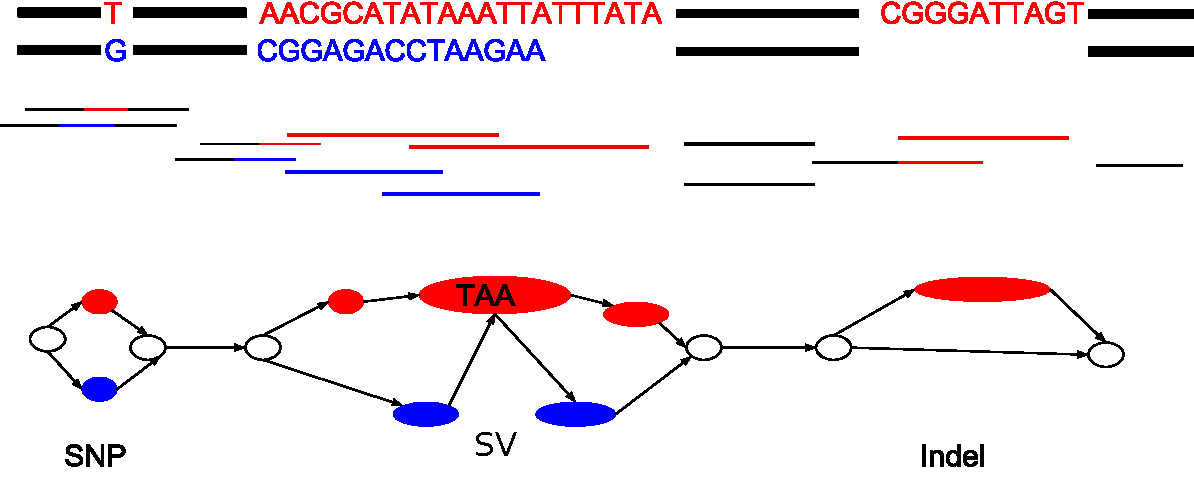
\includegraphics[width=\columnwidth]{ex_sv.pdf}
\caption{Given the input reads (middle) from the two sequences (top), we show a corresponding assembly graph at the bottom.
The bubbles in the sequence graph (bottom) show three different heterozygous variations; the first one is an SNV, the second one is an SV, and the third one is an indel. }
\label{fig:ex_sv}
\end{figure}

\paragraph{De Bruijn graphs.}
% https://genome.sph.umich.edu/w/images/b/b4/666.2012.01.pdf
The de Bruijn graph is a directed graph representing overlaps
between sequences of symbols, named after Nicolass Govert de Bruijn \citep{todd1933combinatorial}. 
In this type of assembly graph, each read is broken into a sequence of overlapping $k$-mers, where a $k$-mer is a substring of length $k$. The distinct
$k$-mers are added as vertices to the graph, and $k$-mers with $k-1$ overlap are connected by an edge.
In Figure~\ref{fig:assembly_graphs}a, the reads are divided into words of fixed length $k$, where $k=4$. Here,
each node in the graph is a word and the connections between the nodes are based on the overlap between nodes.

% Given an
% alphabet $\sigma$ of $n$ symbols, a $k$ dimensional de Bruijn graph has the following properties.
% \begin{enumerate}
%  \item $n^k$ vertices produced by all words of length $k$ from alphabet $\sigma$
%  \item Two vertices X and Y are connected if and only if the $k$ - 1
% suffix of X is equal to the $k$ - 1 prefix of Y.
% \end{enumerate}

The first application of the de Bruijn graph in genome assembly was introduced in
the EULER assembler \citep{pevzner2001eulerian}. 
The assembly problem can then be formulated as finding a walk
through the graph that visits each edge in the graph once --- an Eulerian path problem.
Due to the repeats, it is difficult to find Euler paths. 
In most instances, the assembler attempts to construct
contigs consisting of the unambiguous, unbranching regions of the graph.

\cite{medvedev2007computability}
extended the original directed 
de  Bruijn  graph  model  of  \cite{pevzner2001eulerian}  to  a  bi-directed  
de  Bruijn  graph  (BDDG)  model,  which  is  more  efficient in 
handling DNA’s double-strand structure.  
A bi-directed graph is a generalized directed graph in the 
sense  that  two  end-points  of an  edge  are  given  independent  
orientations  (or  directions)  at   each  end. 
 Thus,  from  sequencing  reads $ R  =  \{R_1,  R_2,  ...  R_m\}$,  we  can  
generate a bi-directed de Bruijn graph by defining the 
vertices  as  $k$-mers  obtained  
from  the  reads  and  then  getting  
all possible edges among the vertices. 


The  advantage  of  BDDG  over  directed  de Bruijn  graph  is  simplification.  Both  strands  of  a  $k$-mer  are  
represented   by   one   node   in   BDDG   compared   to   two   
separated  nodes  in  directed  graph.  For example, if forward strand is represent by node n, then the reverse strand is represented by n' within the same node n.
This saves memory and storage but also simplifies the graph so that graph operations are more efficient.

\paragraph{De Bruijn graph and overlap graph.}
The de Bruijn graph theoretically achieves
the same tasks that the overlap graph does, but in an efficient manner \citep{li2012comparison}.
The de Bruijn graph became widely for assembling the short reads. The OLC
approach did not scale well on the high number of sequences generated by NGS. The
use of the de Bruijn graph is prevalent for short read assembly because these approaches employ efficient techniques to handle redundancy in data. Indeed a k-mer
present multiple times in the sequencing dataset appears only once in the graph. This
makes the de Bruijn graph structure not very sensitive to high coverage, unlike
OLC. The de Bruijn graph was first proposed as an alternative structure \citep{pevzner2001eulerian} because it
was less sensitive to repeats. 

% From the above, it follows that the assembly graphs contain the information about ordering of reads. 
We now discuss the special structures in assembly graphs, that can occur due to repeats and heterozygous regions.

\paragraph{Graph structures.} We discuss mainly two types of structures (bubbles and repeats) that occur in the assembly graphs for diploid genomes.

\textit{Bubbles.}
Bubbles are defined as a set of disjoint paths bounded by a fixed start and an end node and all paths through the bubble flow from start to end. 
No other vertex in the graph other than a start node forms a pair with an end node.
Bubbles in the graph represent heterozygosity or sequencing errors for the diploid organism.
Bubbles can contain simple SNVs with only one bp difference, or even large complex structural variations in the order of kilo-bases or more.  
Figure~\ref{fig:ex_sv} illustrates how bubbles in an assembly graph can contain both small structural variants and large structural variants.
\begin{figure}[t!]\centering
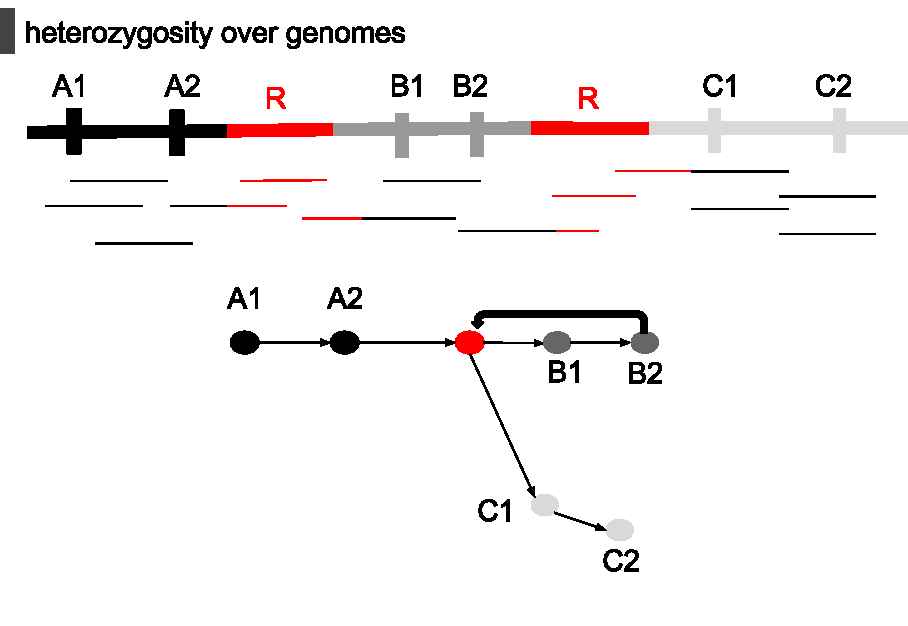
\includegraphics[width=\columnwidth]{repeats.pdf}
\caption{The assembly graph in which repetitive and heterozygous regions are condensed as nodes, is shown. 
At the top, heterozygosity (in vertical bars) and repetitive regions (in red) over the genome are shown. 
At the bottom, the graph with nodes as heterozygous or repetitive region are shown, and connections are based on the successive read overlap.
The graph has cycles because of repetitive region shown by R, which also causes two branches.}
\label{fig:repeats}
\end{figure}

\textit{Repeats.} Repeats in a genome causes branches or cycles in the assembly graphs and, therefore, make a graph more complex and break the properties of the linear reference.
Specifically, it becomes difficult to find the positioning or linear ordering of nodes in the graph.
The repeats in the graph are illustrated in Figure~\ref{fig:repeats}. In this example, the repeat $R$ causes cycles and branches in the graph.
Assemblers generally handle these repeats by making a greedy guess as to which branch to follow.
Incorrect guesses create false joins (chimeric contigs) and erroneous copy numbers. 
If the assembler is more conservative, it will break the assembly at these branch points, leading to an accurate but fragmented assembly with fairly small contigs.
The ability to resolve repeats depends on the reads length. If there is a read that is long enough to span the repeat region, then the repeat is resolvable.
Therefore, upcoming long-read sequencing technologies produce reads that span these repeats helps in obtaining maximally repeat-resolved diploid assemblies.

% We have explored the assembly graphs and their special structures. We now provide the main approaches followed for reconstructing the genome from NGS data. 
\subsection{Related work on diploid assembly}
Over the last decade, the development of various NGS technologies has impacted the assembly problem.
\vspace{10cm}
In theory, the problem of \textit{de novo assembly}---computing the consensus of two or more sequences---is NP-hard, when the problem is modeled either as string graphs or de Bruijn graphs \citep{medvedev2007computability}. 
There are several heuristic approaches for approximating the optimal \textit{de novo} haploid assembly based on NGS datasets \citep{idury1995new, myers1995toward, myers2005fragment, pevzner2001eulerian, nagarajan2009parametric, nagarajan2013sequence, sovic2013approaches}.

However, even with Sanger (reads of the order of 800-1000 base pairs) and Illumina sequencing, which deliver short reads with low error rates, de novo assembly of heterozygous diploid genomes has been a difficult problem \citep{vinson2005assembly, levy2007diploid}.
In practice, there are several short-read assemblers based on Illumina data for heterozygous genomes \citep{kajitani2014efficient, pryszcz2016redundans, simpson2012efficient, bankevich2012spades, li2015fermikit}.
The assemblies that they produce are accurate, but contain gaps and are composed of relatively short contigs and scaffolds. 
Third generation sequencing technologies such as methods available from Pacific Biosciences (PacBio) and Oxford Nanopore Technologies (ONT) deliver much longer reads, but with high error rates.
There are now several long-read assemblers \citep{koren2017canu, vaser2017fast, xiao2016mecat, berlin2015assembling, chin2013nonhybrid, hunt2015circlator, lin2016assembly} that use these long-read data for de novo assembly.
The assemblies that are delivered from these assemblers are more contiguous, with longer contigs and scaffolds.
Finally, there are hybrid assemblers that take advantage of long-read data (with its high error rate) and short-read data (with its low error rate) \citep{bashir2012hybrid, antipov2015hybridspades, zimin2017hybrid} and attempt to combine the best aspects of both.
These hybrid assemblers delivers highly accurate, repeat-resolved assemblies.

The main drawback of the state-of-the-art assemblers mentioned above is that they generate only one consensus sequence even for diploid organisms. To date, there is only one assembler that can produce diploid assemblies for diploid genomes.

\textit{Diploid assembly.} A recent and currently only available diploid assembly method --- Falcon Unzip \citep{chin2016phased} --- is a purely PacBio based diploid assembler.
Falcon Unzip generates haplotype contigs or ``haplotigs'' that represent the diploid genome with correctly phased homologous chromosomes.
Falcon Unzip involves constructing a string graph from long PacBio reads, and generating haplotigs in a greedy manner using a local conservative approach.


For generating haplotigs, Falcon Unzip first identifies the phase for each read based on the condition that the read covers at-least one SNV for phasing.
In the regions over the genome where heterozygous SNVs are at a long distance from each other, Falcon Unzip can not phase those regions, resulting in incomplete assemblies.
Additionally, Falcon Unzip has limitations with respect to phasing all large structural variants and regions with high heterozygosity. 

% The pipeline is given in Figure~\ref{fig:falcon_unzip}.
% Falcon Unzip begins by using reads to construct a string graph that contains sets of ``haplotype-fused contigs'' , also called as ``primary contigs'', as well as bubbles representing divergent regions between homologous sequences (Fig.~\ref{fig:falcon_unzip}a). 
% Next, Falcon-Unzip identifies read haplotypes using phasing information from heterozygous positions that it identifies (Fig.~\ref{fig:falcon_unzip}b). 
% Phased reads are then used to assemble haplotigs and primary contigs (backbone contigs for both haplotypes) (Fig.~\ref{fig:falcon_unzip}c) 
% that form the final diploid assembly with phased single-nucleotide polymorphisms (SNPs) and structural variants (SVs).
% 
% \textit{Phasing using primary contigs.}
% In Falcon Unzip, the reads are aligned to primary contigs and heterozygous SNPs (het-SNPs) are called by analyzing the base frequency of the detailed sequence alignments.
% A simple phasing algorithm was developed to identify phased SNPs. 
% Along each contig, the algorithm assigns phasing blocks where ``chained phased SNPs'' can be identified. 
% Within each block, if a raw read contains a sufficient number of het-SNPs, it assigns a haplotype phase for the read unambiguously. 
% Combined with the block and the haplotype phase information, it assigns a ``block-phase'' tag for each phased read in each phasing block.
% Some reads might not have enough phasing information. For example, if there are not enough het-SNP sites covered by a read, it assigns a special 'un-phased tag' for each un-phased read.
% The initial assembly graph is fused using phased reads and the haplotigs are generated in a greedy manner using local conservative approach.
% % \todo{maybe add example how haplotigs from haplotype fused assembly graph works?}

% \begin{figure}[t!]\centering
% \includegraphics[width=\columnwidth]{{cropped_falcon-unzip}.pdf}
% \caption{(a) An initial assembly is computed by FALCON, which error corrects the raw reads (not shown) and then assembles them using a string graph of the read overlaps. 
% The assembled contigs are further refined by FALCON-Unzip into a final set of contigs and haplotigs. 
% (b) Phase heterozygous SNPs and group reads by haplotype. (c) The phased reads are used to open up the haplotype-fused path and generate as output a set of primary contigs and associated haplotigs.}
% \label{fig:falcon_unzip}
% \end{figure}

There is no known algorithm that works at different levels of heterozygosity, phases all types of structural variants and generates complete diploid assemblies.
A potential approach to achieve the task of complete diploid genomes is to perform phasing directly on the assembly graph.
Moreover, it becomes easy to detect large structural variants, such as translocations and other rearrangements, in an assembly graph.
Thus, working in the space of assembly graphs provides the opportunity to detect all types of structural variation, which further helps in phasing whole genomes.

Additionally, Falcon Unzip is purely relying on PacBio data, which is noisy and, therefore, it requires high coverage data for producing accurate assemblies.
In contrast, hybrid approaches that combine accurate Illumina and long read PacBio data, conceptually have the potential for producing good quality assemblies even at low coverages.
However, there is no known algorithm that combines multiple sequencing datasets such as accurate Illumina and long read PacBio data for producing good quality haplotigs.
\begin{gaps}
 Phasing bubbles directly from the assembly graph is an open problem. Additionally, the extension to MEC formulation for phasing reads mapped to assembly graphs do not exist. 
 \label{gap:gap4}
\end{gaps}


% \begin{figure}[t!]\centering
% 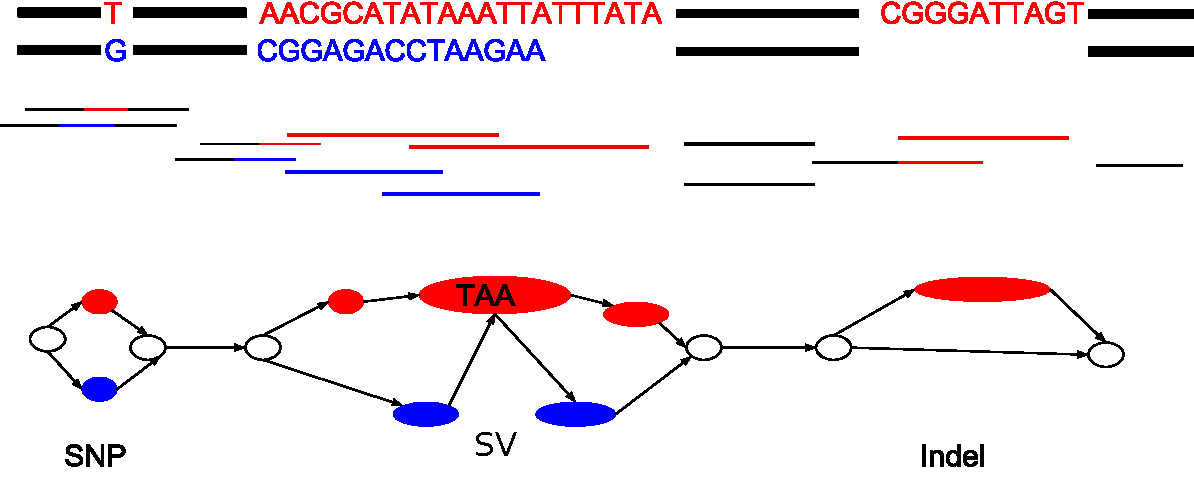
\includegraphics[width=\columnwidth]{ex_sv.pdf}
% \caption{Based on reads (middle) from the two sequences (top), the bubbles in the graph (bottom) show three different heterozygous structural variations; first is a SNV, second is a SV and third is an indel. }
% \label{fig:ex_sv}
% \end{figure}
\section{Thesis Scope and Outline}
In the above sections, I highlighted four ``open problems'' in the area of haplotyping using NGS data.
The remainder of this thesis is structured as follows:

\begin{itemize}
 \item Chapter 2 provides a general background on the different types of algorithms. 
 It establishes the motivation on how these algorithms are used in solving small daily examples fast. 
 It highlights the advantages and disadvantages of these algorithms in context of large problems.
 \item Chapter 3 presents a dynamic programming based algorithm for solving \GMEC instances approximately.
 It discusses the approximation guarantee, that provides hint about the existence of polynomial time approximation scheme for these instances. (Problem~\ref{gap:gap1})
  \item Chapter 4 discusses different types of NGS datasets, with their advantages and disadvantages. 
  It explores an integrative phasing framework that is obtained for combining NGS datasets. 
  It discusses a parameterized algorithm that solves these instances efficiently in practice. 
  Furthermore, I demonstrate the effectiveness of this algorithm on real genomic datasets. (Problem~\ref{gap:gap2})

 \item Chapter 5 presents a generalized parameterized approach to incorporate information from pedigrees. 
Furthermore, I show experiments on real datasets and highlight that pedigree data has an additional advantage in delivering better quality haplotypes. (Problem~\ref{gap:gap3})
  \item Chapter 6 focuses on a generalized approach --- haplotype-aware diploid assembly --- in a graph framework, that has the ability to handle all levels of heterozygosity and structural variations to produce accurate and complete haplotype assemblies.
 Furthermore, I present this approach as a hybrid of different types of NGS datasets and show its effectiveness on a pseudo-diploid genome. (Problem~\ref{gap:gap4})

 \item Finally, Chapter 7 summarizes the results presented in this thesis, along with an outlook into the future and perspectives.
\end{itemize}

\section{Relevant publications}
\begin{itemize}
 \item David Porubsky*, \underline{Shilpa Garg}*, Ashley D. Sanders*, V. Guryev, Peter M. Lansdorp, T. Marschall,
\textit{Dense And Accurate Whole-Chromosome Haplotyping Of Individual Genomes}, Nature Communications, 2017.


\item \underline{Shilpa Garg}, Marcel Martin and Tobias Marschall, \textit{Read-Based Phasing of Related Individuals},
Proceedings of ISMB 2016/Bioinformatics.
\item \underline{Shilpa Garg}, Mikko Rautiainen, Adam M Novak, Erik Garrison, Richard Durbin, Tobias Marschall, \textit{A graph-based approach to diploid genome assembly}, ISMB 2018 (to appear).
\item Preprint: \underline{Shilpa Garg}, Tobias Moemke, \textit{A QPTAS for Gapless-MEC}, Submitted.
\item Preprint: M. Martin*, M. Patterson*, \underline{Shilpa Garg}, S. O. Fischer, N. Pisanti, G. W. Klau, A. Schnhuth, T.
Marschall, \textit{WhatsHap: fast and accurate read-based phasing}.

In this paper, my contribution was in developing some parts of the pipeline and making figures.
\end{itemize}


% \subsection{Issues we address}
% To address those problems, we will present new algorithmic approaches. 
% \begin{itemize}
% \item In the second chapter, we present the fundamental concepts of different type of algorithms.
%  \item In the third chapter, we present dynamic programming based algorithm to prove the near-polynomial approximation status of \GMEC.
%  \item In the forth chapter, we present a parameterized algorithm to solve \MEC instances integatively from different datasets.
%   \item In the fifth chapter, we present a integrative framework to solve sequencing-based and genetic haplotyping, helps to generate complete and accurate haplotypes.
%  \item In the sixth chapter, we introduce new way to represent the assembly graph and futher, finding long read paths in the graph based on different types of datasets, which futher helps in better phasing. 
% \end{itemize}


% 
% 
%  
% 
% \todo{cover these issues in approaches}
% \subsection{Diploid genome assembly hardness}
% \begin{itemize}
% \item Theoretical approximation gurantee on gapless-MEC. It is important because even for high coverages, we can solve it in polynomial time approximately.
%  \item integrating datasets to produce more accurarte and complete
%  \item non-reference denovo based, can not detect large SVs, directly from graph, hybrid
%  \item pedigree of genomes
% \end{itemize}
% 
% \subsection{Goals and achievements}
% \begin{enumerate}
%  \item DNA genomes ranging from small yeast like genome to larger ones like human.
%  \item end-to-end full genome sequences
%  \item efficient algorithms to generate optimal or near-optimal solution.
% \end{enumerate}
% 
% 
% 
% 
% \subsection{Outline of our contributions}
% \begin{enumerate}
%  \item Chpater 1 consists of ...
%   \item Chpater 2 consists of ...
%    \item Chpater 3 consists of ...
% \end{enumerate}






